% planisphere.tex
%
% The LaTeX code in this file brings together into a single document the
% various components of the model planisphere.
%
% Copyright (C) 2014-2020 Dominic Ford <dcf21-www@dcford.org.uk>
%
% This code is free software; you can redistribute it and/or modify it under
% the terms of the GNU General Public License as published by the Free Software
% Foundation; either version 2 of the License, or (at your option) any later
% version.
%
% You should have received a copy of the GNU General Public License along with
% this file; if not, write to the Free Software Foundation, Inc., 51 Franklin
% Street, Fifth Floor, Boston, MA  02110-1301, USA

% ----------------------------------------------------------------------------

\documentclass[a4paper,onecolumn,10pt]{article}
\usepackage[dvips]{graphicx}
\usepackage{fancyhdr,url}
\usepackage[utf8]{inputenc}
\usepackage{parskip}
\usepackage[pdftitle={Fabriquer son cherche-etoiles}, pdfauthor={Dominic Ford}, pdfsubject={Fabriquer son cherche-etoiles}, pdfkeywords={Fabriquer son cherche-etoiles}, colorlinks=true, linkcolor=blue, citecolor=blue, filecolor=blue, urlcolor=blue]{hyperref}
\usepackage[T1]{fontenc}
\renewcommand{\familydefault}{\sfdefault}
\pagestyle{fancy}

\lhead{\it Fabriquer son cherche-étoiles}
\chead{}
\rhead{\thepage}
\lfoot{}\rfoot{}
\cfoot{\bf\footnotesize\copyright\ 2014--2020 Dominic Ford. Distribué sous licence publique générale GNU version 3. Document téléchargé depuis \url{https://in-the-sky.org/planisphere/}}

\fancypagestyle{plain}{%
\fancyhf{} % clear all header and footer fields
\renewcommand{\headrulewidth}{0pt}
\renewcommand{\footrulewidth}{0pt}}

\title{Fabriquer son cherche-étoiles}
\author{Dominic Ford}
\date{2014--2020}

\begin{document}
\maketitle
\setcounter{footnote}{1}

Un cherche-étoiles est un accessoire de poche simple fournissant une carte des étoiles visibles dans le ciel à n’importe quel instant. Au moyen d’un disque rotatif, il montre comment les étoiles se déplacent dans le ciel pendant la nuit et la manière dont différentes constellations sont visibles selon la période de l’année.

On peut se fabriquer son cherche-étoiles en papier ou en carton à l’aide du matériel ci-dessous.

\section*{Ce dont vous avez besoin}

\begin{itemize}
\item Deux feuilles A4 de papier ou de carton fin.
\item Des ciseaux.
\item Une attache parisienne.
\item Facultatif: une feuille de plastique transparent, par exemple en acétate comme celles que l’on utilise pour les rétroprojecteurs.
\item Facultatif: un peu de colle.
\end{itemize}

\section*{Instructions}

{\bf Étape 1} -- Les cherche-étoiles ont une apparence légèrement différente selon le lieu où l’on vit. Celui que nous proposons ici est destiné à être utilisé à n’importe quel endroit de la Terre situé à une latitude de \input{tmp/lat}. Si vous vivez ailleurs, vous pourrez trouver des versions prévues pour n’importe quelle autre latitude à l’adresse

\centerline{\tt https://in-the-sky.org/planisphere}

{\bf Étape 2} -- Imprimez les pages de ce PDF où figurent le disque de la carte du ciel et la partie principale du cherche-étoiles sur deux feuilles distinctes, en papier ou en carton fin de préférence.

{\bf Étape 3} -- Découpez soigneusement le disque de la carte du ciel et la partie principale du cherche-étoiles. Découpez aussi la zone grisée de cette dernière, et si vous l’avez, la grille imprimée sur un transparent. Si vous utilisez du carton, il est peut-être préférable d’inciser légèrement la partie principale le long des pointillés pour pouvoir la plier plus facilement par la suite.

{\bf Étape 4} -- Au centre du disque de la carte du ciel se trouve un petit cercle auquel correspond un autre petit cercle en bas de la partie principale du cherche-étoiles. Percez un petit trou (2\,mm de diamètre environ) dans ces deux éléments. Une perforatrice est l’outil idéal si vous en avez une, sinon utilisez une pointe de compas et agrandissez le trou par un mouvement circulaire.

{\bf Étape 5} -- Introduisez une attache parisienne au centre du disque de la carte du ciel, avec la tête de l’attache du côté de la face imprimée. Ensuite, placez la partie principale du cherche-étoiles sur la même attache avec la face imprimée contre l’arrière de l’attache. Écartez et rabattez les lamelles de cette dernière pour fixer ensemble les deux morceaux de carton.

{\bf Étape 6 (Facultatif)} -- Si vous avez imprimé la dernière page du PDF sur une feuille de plastique, c’est le moment de coller cette grille par-dessus la fenêtre de visualisation que vous avez découpée dans la partie principale du cherche-étoiles.

{\bf Étape 7} -- Pliez la partie principale du cherche-étoiles le long des pointillés de manière à ce que l’ouverture que vous y avez pratiquée permette de voir la face imprimée du disque de la carte du ciel.


{\bf Félicitations, votre cherche-étoiles est maintenant prêt à être utilisé!}

\section*{Comment s’utilise un cherche-étoiles?}

Tournez le disque de la carte du ciel jusqu’à trouver sur son pourtour le point où est inscrite la date du jour et alignez ce point avec l’heure actuelle. La fenêtre de visualisation montre maintenant toutes les constellations visibles dans le ciel.

Allez dehors et tournez-vous vers le nord. Si vous tenez le cherche-étoiles à bout de bras vers le ciel, les étoiles figurant au bas de la fenêtre de visualisation doivent coïncider avec celles que vous voyez dans le ciel face à vous.

Tournez-vous vers l’est ou l’ouest, et faites pivoter le cherche-étoiles de sorte que le mot \guillemotleft Est\guillemotright\ ou \guillemotleft Ouest\guillemotright\ soit en bas de la fenêtre. Là encore, les étoiles dans la partie inférieure de la fenêtre de visualisation doivent correspondre à celles que vous voyez devant vous dans le ciel. 

Si vous avez imprimé la grille des lignes d’altitude et d’azimut sur un transparent, celles-ci vous permettent de déterminer à quelle hauteur les objets apparaissent dans le ciel et dans quelle direction. Les cercles sont dessinés à des altitudes de 10, 20, 30...80 degrés au-dessus de l’horizon. À titre de comparaison, une distance de 10$^\circ$ équivaut à peu près à la largeur de la main lorsqu’on tend le bras. Les lignes courbes sont des verticales reliant des points sur l’horizon au point situé juste au-dessus de votre tête. Elles sont placées aux points cardinaux S, SSE, SE, ESE, E, etc.


\section*{License}

Comme tout ce qui se trouve sur In-The-Sky.org, les droits pour ce cherche-étoiles à monter sont la propriété de Dominic Ford. Cependant, le contenu de In-The-Sky.org est intégralement mis à la disposition des astronomes amateurs du monde entier, et vous êtes libre de modifier et/ou de redistribuer n’importe quelle partie de ce site aux conditions suivantes: (1) Tout élément accompagné d’une mention copyright doit inclure cette mention non modifiée dans votre version redistribuée, (2) Vous devez m’attribuer à moi, Dominic Ford, la qualité d’auteur et de détenteur du copyright (3) Vous n’êtes pas autorisé à tirer profit de la reproduction des contenus de ce site sauf si vous êtes une organisation à but non lucratif officielle ayant précisément pour objet le progrès scientifique dans le domaine de l’astronomie, ou que vous avez la permission écrite de l’auteur.

\newpage

\centerline{\includegraphics{tmp/starwheel}}

\vspace{1cm}
La carte du ciel, partie centrale du cherche-étoiles à insérer dans la pochette.

\newpage
\thispagestyle{empty}
\vspace*{-3.0cm}
\centerline{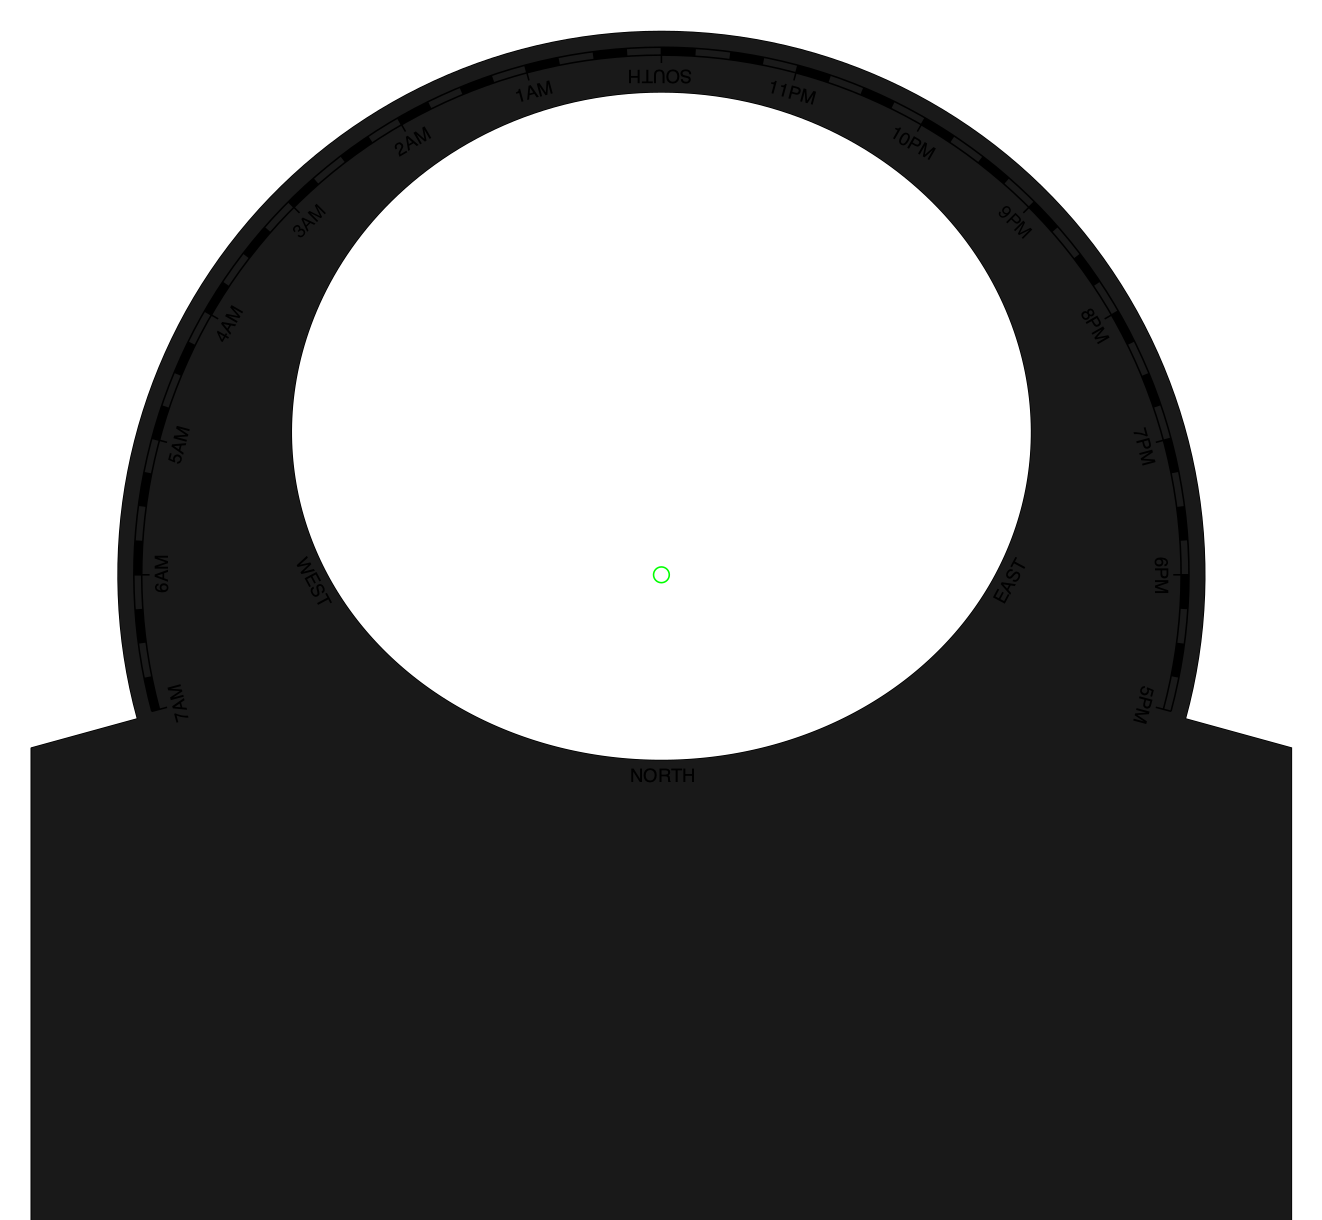
\includegraphics{tmp/holder}}
\newpage

\centerline{\includegraphics{tmp/altaz}}

\vspace{1cm}
Cette grille peut éventuellement être imprimée sur du plastique transparent et collée sur l’ouverture pratiquée dans le cadre du cherche-étoiles pour afficher les altitudes des objets dans le ciel et leur orientation.

\end{document}

